\documentclass[11pt]{article}

\usepackage{url,amsmath,mathtools,bbm,amsthm, amssymb, fourier, dsfont, listings, cases,  subcaption}
\usepackage{graphicx}
\usepackage{listings}
\usepackage[margin=1.15in]{geometry}

\usepackage[dvipsnames]{xcolor}
\usepackage[shortlabels]{enumitem}
\newcommand{\note}[1]{{\leavevmode\color{BrickRed}{#1}}}

\newcommand{\E}{\mathbbm{E}}
\newcommand{\R}{\mathbbm{R}}
\newcommand{\N}{\mathbbm{N}}
\newcommand{\mathd}{\mathrm{d}}
\newcommand{\dx}[1]{\,\mathd #1}
\newcommand{\norm}[1]{\left\lVert#1\right\rVert}

\newtheorem{theorem}{Theorem}

\begin{document}

\title{Homework 3\\MATH 6610-001, Fall 2019}
\author{Placede Tshiaba}
\maketitle

\section*{Problem assignment}
\subsection*{Lecture 20 \#20.1}
Let $ A \in \mathbb{}^{m \times m}$ be nonsingular. Let's show that $A$ has an $LU$ factorization if and only if for each $1 \le k \le m$, the upper-left $k\times k$ block $A_{1:k, 1:k}$ is nonsingular.\\\\
\underline{\textbf{Solution}}\\
$\implies)$ Let $A \in \mathbb{C}^{m \times m}$ such that has an $LU$ factorization.
\begin{align*}
\begin{bmatrix}
A_{1:k, 1:k} & A_{1:k, k+1:m}\\
A_{k+1:m, 1:k} & A_{k+1:m, k+1:m}
\end{bmatrix}
= 
\begin{bmatrix}
L_{1:k, 1:k} & 0\\
L_{k+1:m, 1:k} & L_{k+1:m, k+1:m}
\end{bmatrix}
*
\begin{bmatrix}
U_{1:k, 1:k} & U_{1:k, k+1:m}\\
0 & U_{k+1:m, k+1:m}
\end{bmatrix}
\end{align*}
So, $ A_{1:k, 1:k}  = L_{1:k, 1:k}*U_{1:k, 1:k} \\
\implies \text{det}(A_{1:k, 1:k}) = \text{det}(L_{1:k, 1:k})*\text{det}(U_{1:k, 1:k}) = \prod\limits_{j=1}^{k}{L_{jj}U_{jj}} =\prod\limits_{j=1}^{k}{U_{jj}} $ because the diagonal elements of $L$ are equal to 1.\\
 $U$ is upper-triangular  with nonzero diagonal elements.Therefore, $\text{det}(A_{1:k, 1:k}) = \prod\limits_{j=1}^{k}{U_{jj}} \ne 0\\
\implies \text{det}(A_{1:k, 1:k}) \ne 0$ and $A_{1:k, 1:K}$ is nonsingular.\\\\
$\Longleftarrow)$  Let's suppose that $\forall k, 1\le k\le m, A_{1:k, 1:k}$ is nonsingular and let's show that A has an $LU$ factorization.\\
We will do a proof by induction.\\
For $\text{dim} (A) =1,\;\; A = (a_{11})$ nonsingular means $a_{11} \ne 0.\;\; A$ has an $LU$ factorization $ A = 1.a_{11}$  where  $L= 1$ and $U = a_{11}.$\\
Let's suppose that for $\text{dim}(A) \le m-1, \;\; A$ has an $LU$ factorization and let's try to find $L, l^T, U, v$ and$ w$ such that

\begin{align*}
\tilde{A} = 
\begin{bmatrix*}
A & b\\
c^T & d
\end{bmatrix*}
=
\begin{bmatrix*}
L & 0\\
l^T & 1
\end{bmatrix*}
*
\begin{bmatrix*}
U & v\\
0 & w
\end{bmatrix*}
\implies
\end{align*}
\begin{numcases}{}
A = LU   \label{eq11}\\
b = Lv     \label{eq12}\\
l^TU = c^T  \label{eq13} \\
l^Tv +w = d   \label{eq14}
\end{numcases}\\
We have $\text{dim}(A) = m-1 \implies A = LU. \; A$ invertible $\implies L$ and $U$ invertible; this implies that we can solve( \ref{eq12}), (\ref{eq13}) and (\ref{eq14}) for $v, l^t$ and $w$. Meaning $\tilde{A}$ has an $LU$ factorization.\\


\noindent Proof that the $LU$ factorization is unique.\\
Let's suppose that A is nonsingular with 2 $LU$ factorizations: $A = L_1U_1$ and $A= L_2U_2$.
\begin{flalign*}
L_1U_1 = L_2U_2 \implies L_2^{-1}L_1U_1 = U_2 \implies L_2^{-1}L_1=U_2^{-1}U_1^{-1} &&
\end{flalign*}
$L_2^{-1}L_1$ is lower-triangular because the inverse of a lower-triangular matrix is lower-triangular and the product of 2 lower-triangular matrices is a lower-triangular matrix.\\
Also, $U_2U_1^{-1}$ is upper- triangular because the inverse of an upper-triangular matrix is upper-triangular and the product of 2 upper-triangular matrices is an upper-triangular matrix.\\
Therefore, $L_2^{-1}L_1$ and $U_2U_1^{-1}$ are diagonal matrices.\\
$L_2^{-1}L_1$ diagonal matrix $\implies L_2^{-1}L_1= I_{m \times m}\implies  L_2 =  L_1.$ Also, $U_2U_1^{-1} = I_{m \times m} \implies U_2=U_1$.\\
In conclusion, $L_1U_1 = L_2U_2.$  If A is nonsingular, A has an unique LU factorization.


\subsection*{Lecture 21 \#21.6}
Suppose $A \in \mathbb{C}^{m \times m}$ is strictly column diagonally dominant, which means for each $k$,
\begin{equation*}
\left|a_{kk}\right|> \sum\limits_{j \ne k}{\left|{a_{jk}}\right|}
\end{equation*}
Let's show that if Gaussian elimination with partial pivoting is applied to $A$, no row interchanges take place.\\
\underline{\textbf{Solution}}\\
For the first column of $A, \text{  A strictly column dominant} \implies \;\left| a_{11}\right| > \sum \limits_{j \ne 1}{\left|{a_{j1}}\right|} \;\; \implies  \left| a_{11}\right| = max_{1 \leq i \leq n}
\left| a_{i1}\right|  $; so there is no need to pivot the first row.\\
Let $A^{(k)}$ be the $(n-k) \times (n-k)$ matrix in the lower left corner obtained after the $k^{th}$ round of  Gaussian elimination.\\
It suffices to prove that all the $A^{(k)}$ are diagonally dominant.\\
Let's show that $A^{(1)}$ is diagonally dominant.\\
Let 
\begin{align*}
A = 
\begin{bmatrix}
\alpha & w\\
v &  B
\end{bmatrix}
\end{align*}
One step Gaussian elimination yields:
\begin{align*}
A = 
\begin{bmatrix}
1 & w\\
\frac{v}{\alpha} &  I
\end{bmatrix}
\begin{bmatrix}
\alpha & w\\
0 &  B- \frac{vw}{\alpha}
\end{bmatrix}
\end{align*}

$A^{(1)} =  B- \frac{vw}{\alpha}$.\\\\
Let $a_{ij}^{(1)}$ be the $(i, j)$ entry of $A^{(1)}$.

\begin{flalign*}
\sum\limits_{ i \geq 2, \;\; i\ne j}^ {n}{\left|a_{ij}^{(1)}\right|} & = \sum\limits_{ i \geq 2, \;\; i\ne j}^ {n}{\left|b_{ij} - \frac{v_i w_j}{\alpha}\right|} &&\\
   & \leq  \sum\limits_{ i \geq 2, \;\; i\ne j}^ {n}{\left|b_{ij} \right|} +  \sum\limits_{ i \geq 2, \;\; i\ne j}^ {n}{\left|\frac{v_i w_j}{\alpha}\right|} && \\
   &  < \left|b_{jj} \right| - \left|w_{j} \right| + \frac{\left|w_j\right|}{\alpha}(\left| \alpha\right| - \left|v_j\right|)  \text {  because A is diagonally dominant}&&\\
  &  = \left|b_{jj} \right| - \frac{\left|w_j\right|}{\alpha}\left| v_j\right| &&\\
  & \leq \left| b_{jj} - \frac{w_jv_j}{\alpha}\right| = a_{jj}^{(1)}
\end{flalign*}
This means that $A$ diagonally dominant $\implies A^{(1)}$ diagonally dominant $\implies A^{(2)}$ diagonally dominant$\cdots \implies A^{(k)}$ diagonally dominant.\\
So if the Gaussian elimination is applied to $A$, diagonally dominant, no row interchanges take place.


\subsection*{Lecture 22 \#22.3}
Reproduction of the figures of the $22^{nd}$ lecture of our textbook, approximately if not in full detail,  but based on random matrices with entries uniformly distributed in [-1,1] rather that normally distributed.\\
\underline{\textbf{Solution}}\\
\begin{enumerate}[(a)]
\pagebreak
\item Growth factor versus matrix dimension.
\begin{figure}[htbp]
  \begin{center}
  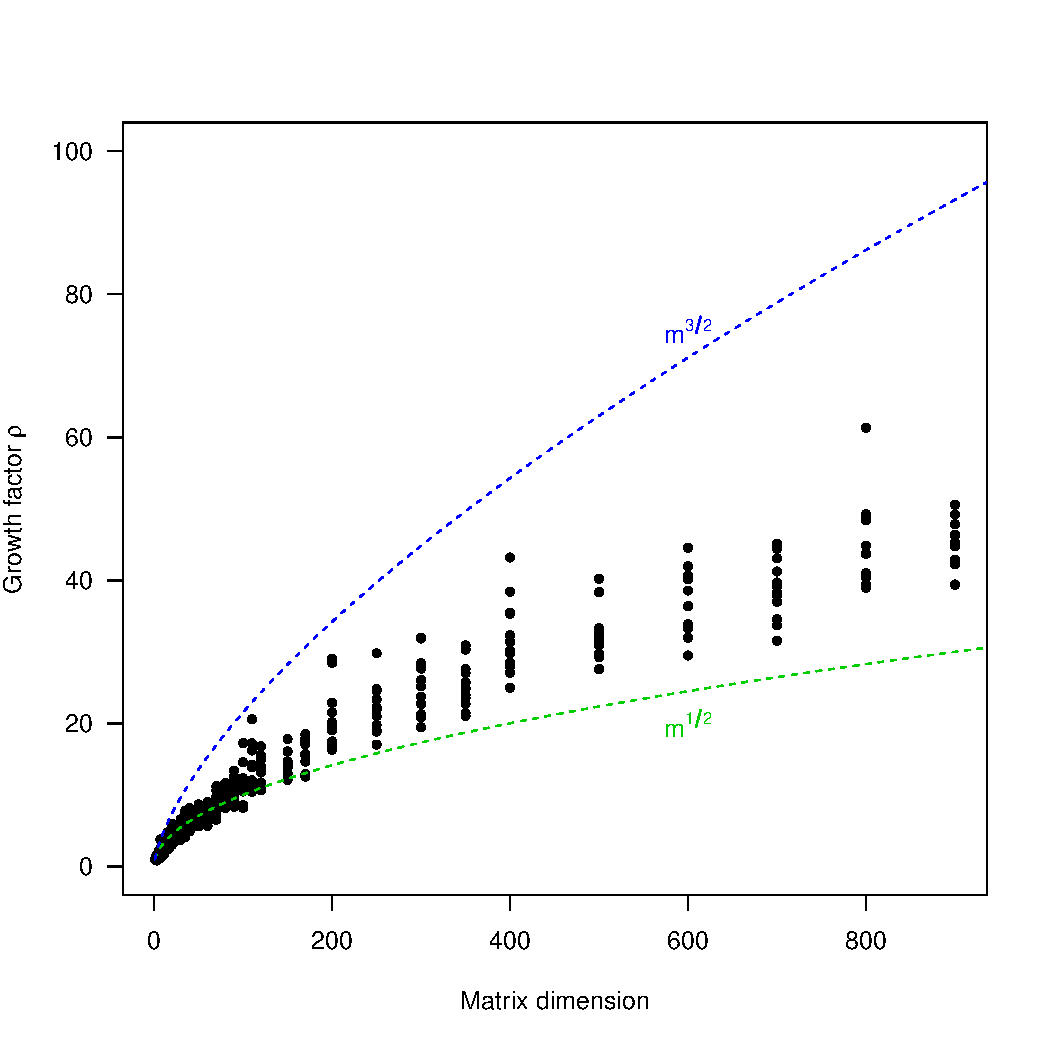
\includegraphics[scale =.8]{growth_factor.pdf}
  \caption{Growth factors for Gaussian elimination with partial pivoting applied to 468 random matrices (independent, entries uniformly distributed on [-1,1])} \label{fig:22.1} 
  \end{center}
\end{figure}\\
Figure~\ref{fig:22.1} shows that when Gaussian elimination with partial pivoting is applied to matrices  with entries from random uniform distributions on [-1, 1], the typical size of $\rho$ is between $m^{1/2}$ and $m^{3/2}$. This is different from what appears in our textbook when the entries of the matrices are chosen from random normal distributions.

\pagebreak
\item Probability density function for growth factors of random matrices
\begin{figure}[htbp]
  \begin{center}
  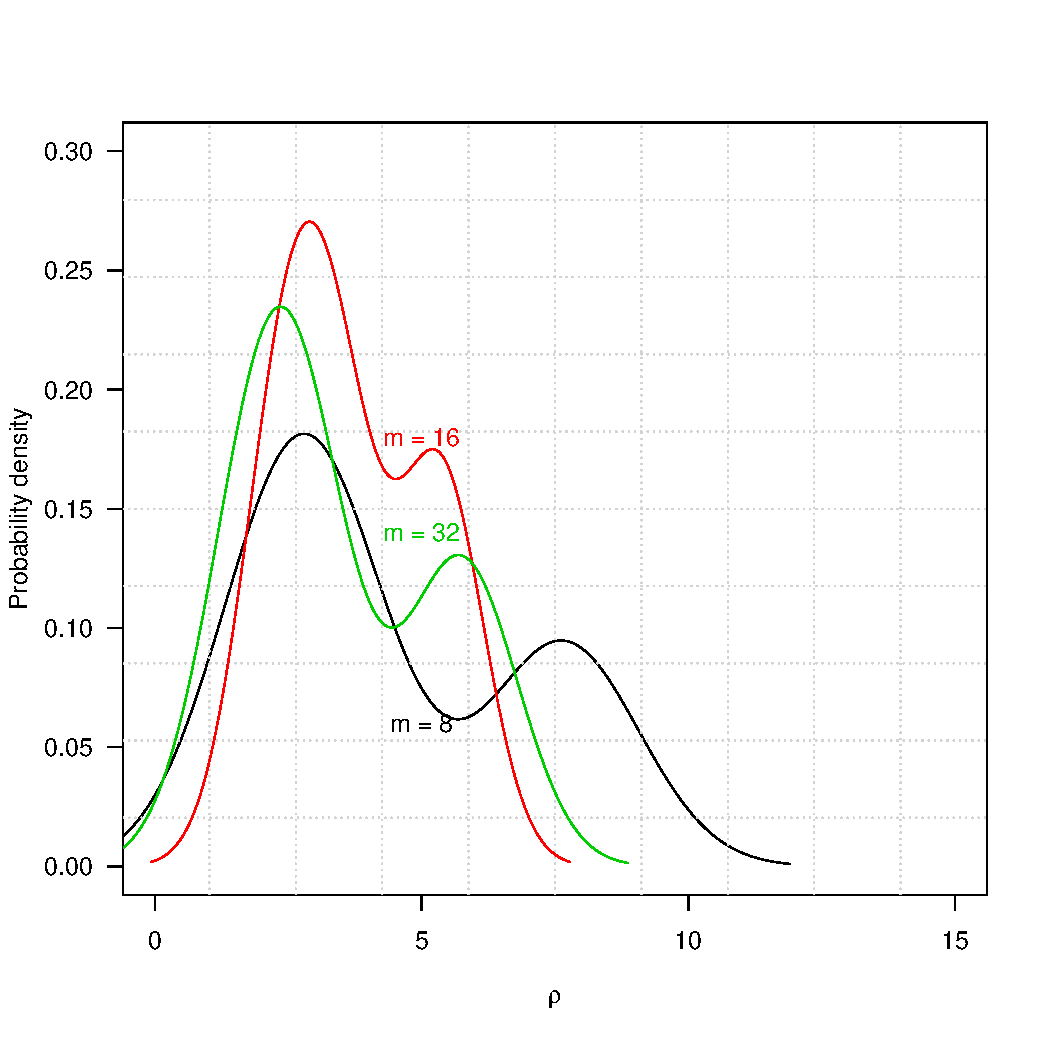
\includegraphics[scale =.8]{probability_density_function.pdf}
  \caption{Probability density distributions for growth factors of random matrices of dimensions  $m =$ 8, 16, 32, based on samples sizes of one million for each dimension} \label{fig:22.2} 
  \end{center}
  \end{figure}\\
The probability density plots show that in each case ($m =$8, 16, 32), the growth factor decreases exponentially with $\rho$. The peaks reflect the fact that the distribution is uniform and not normal.

\pagebreak

\item $PA = LU$ factorization\\
\begin{figure}[h]
\centering
  \begin{subfigure}[b]{0.4\textwidth}
    \begin{center}
    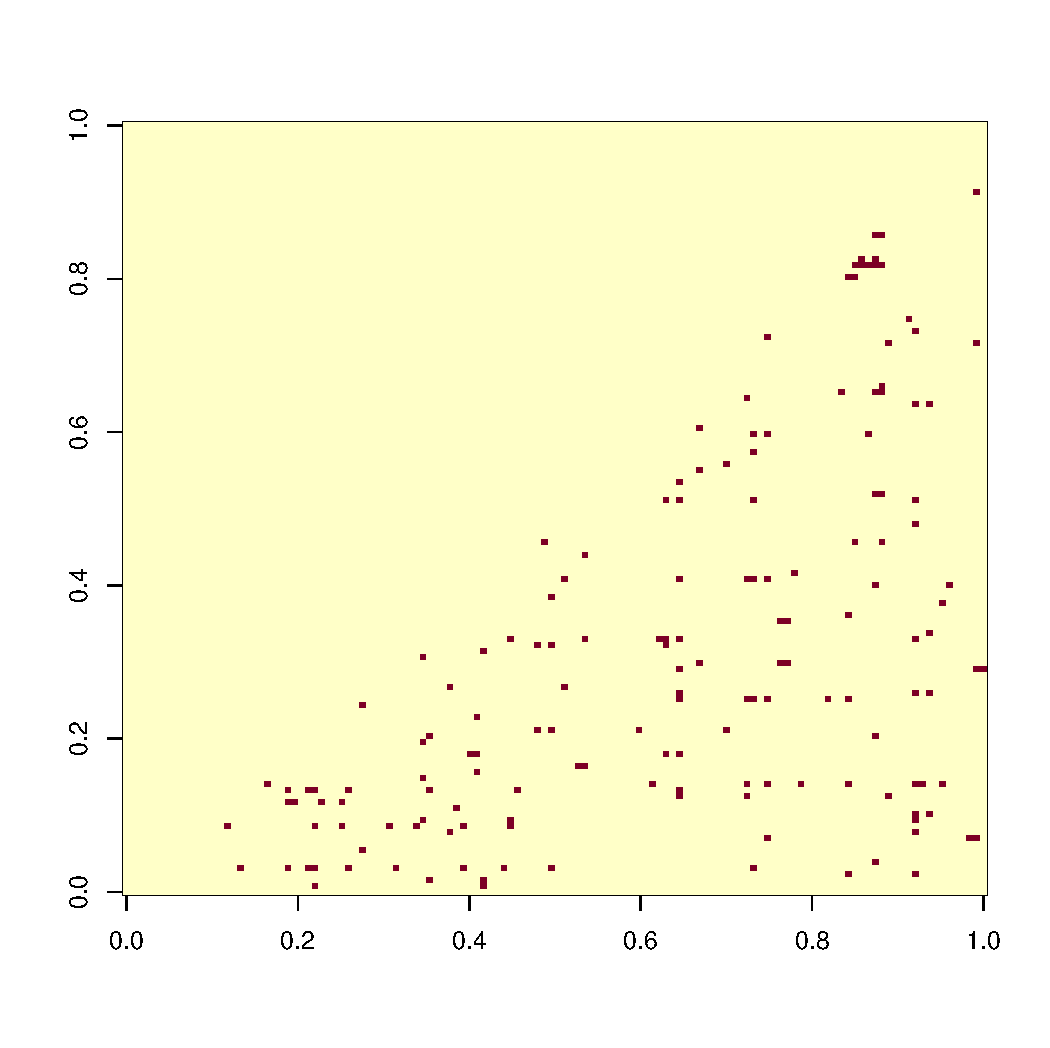
\includegraphics[width=7 cm, clip = false]{Lmatrix1.pdf}
    \caption{random A $ max_{i,j}\left| (L^{-1})_{ij}\right| = 2.49$}
    \label{fig:22.3.a}
    \end{center}
  \end{subfigure}
\hfill
  \begin{subfigure}[b]{0.4\textwidth}
    \centering
    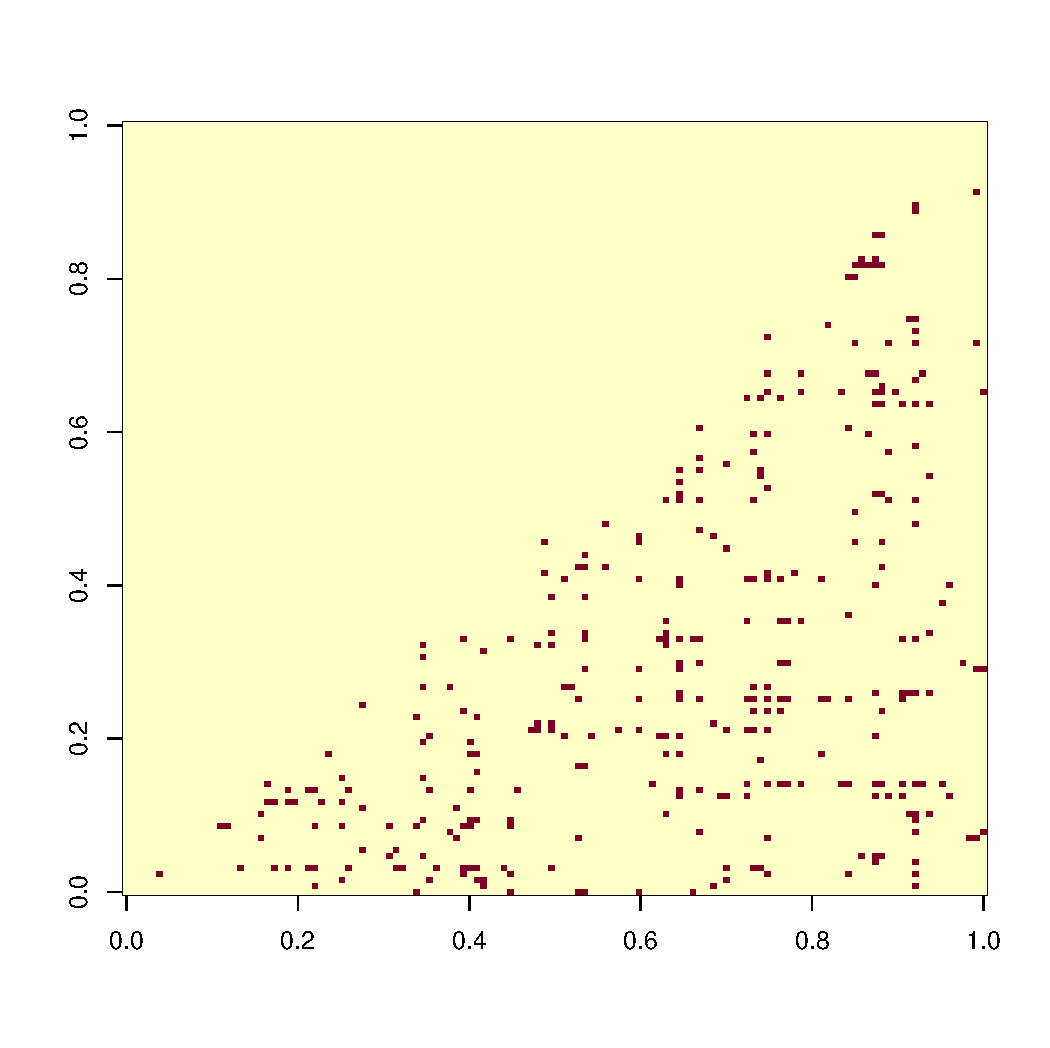
\includegraphics[width = 7 cm]{Lmatrix2.pdf}
    \caption{random $\tilde{L}\max_{i,j} \left| (\tilde{L}^{-1})_{ij}\right| = 2.49$}
    \label{fig:22.3.b}
  \end{subfigure}
 \caption{Let A be a random 128 $\times$ 128 matrix with factorization $PA = LU.$ On the left, $L^{-1}$ is shown: the dots represent entries with magnitude $\geq 1.$ On the right, a similar picture for $\tilde{L}^{-1}$, where $\tilde{L}$ is the same as $L$ except that the signs of its subdiagonal entries have been randomized}\label{fig:22.3}
\end{figure}\\
The plots on figure~\ref{fig:22.3} show that Gaussian elimination tends to produce matrices $L$ that are extraordinarily well-conditioned.

\pagebreak
\item $Q$ portraits of the same two matrices
\begin{figure}[h]
\centering
  \begin{subfigure}[b]{0.4\textwidth}
    \begin{center}
    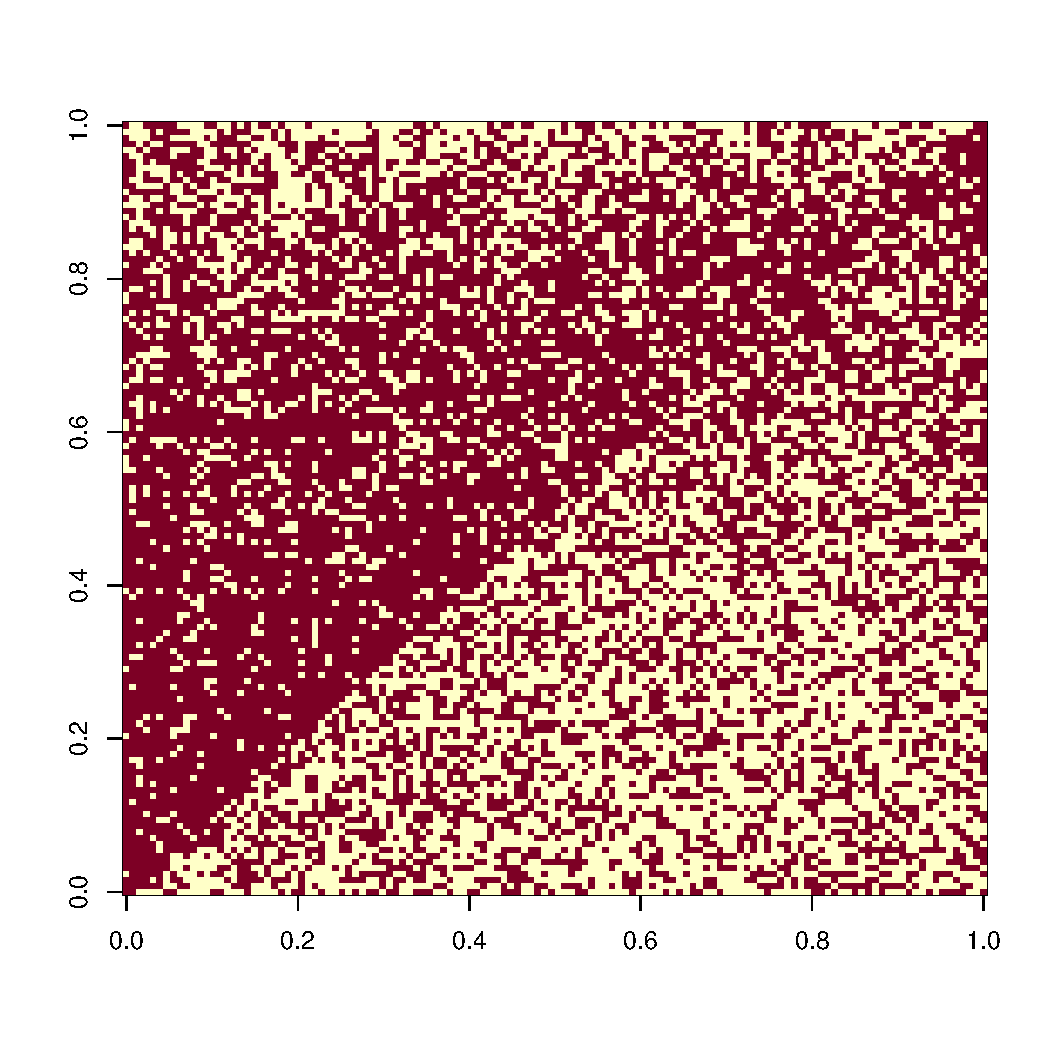
\includegraphics[width=7 cm, clip = false]{randomA.pdf}
    \caption{random A }
    \label{fig:22.4.a}
    \end{center}
  \end{subfigure}
\hfill
  \begin{subfigure}[b]{0.4\textwidth}
    \centering
    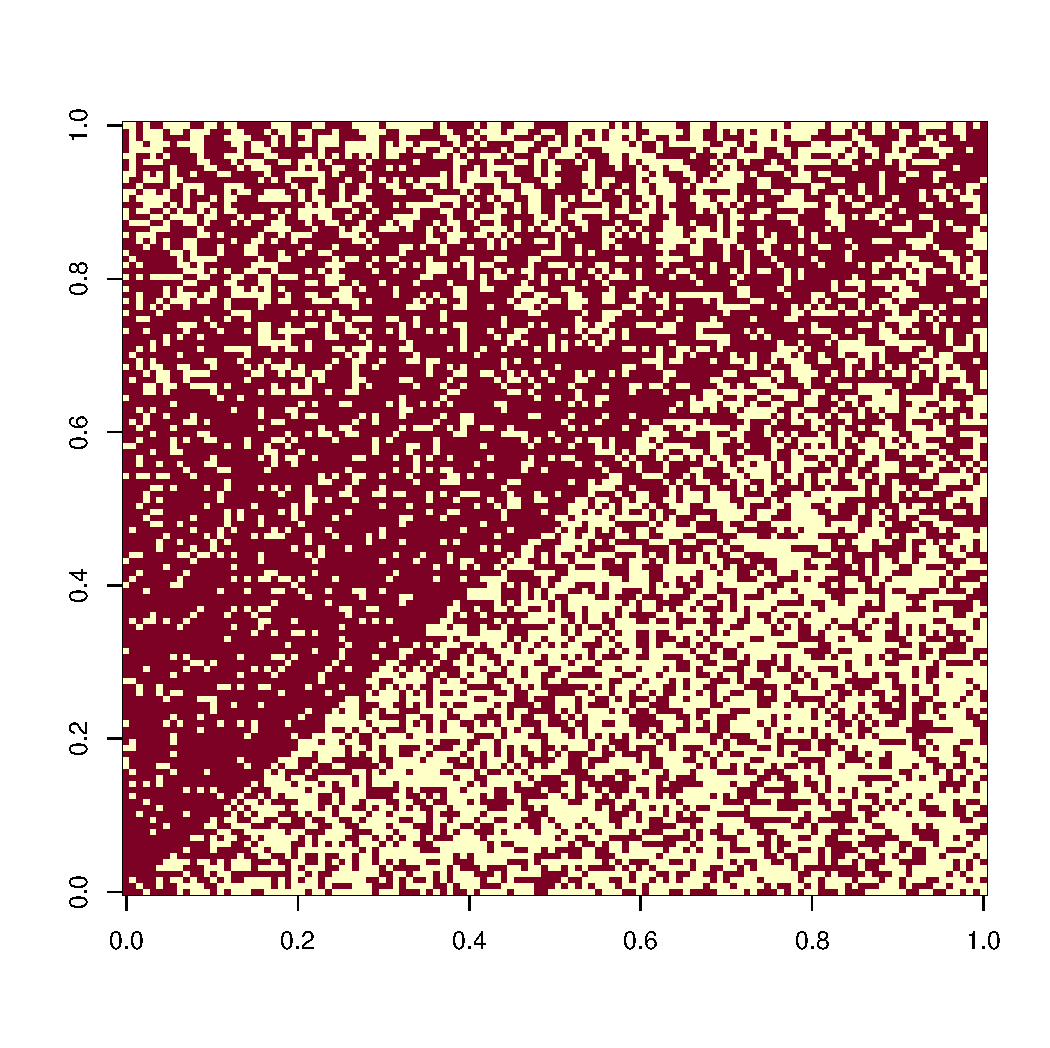
\includegraphics[width = 7 cm]{randomL.pdf}
    \caption{random $\tilde{L}$}
    \label{fig:22.4.b}
  \end{subfigure}
 \caption{On the left, the random matrix $A$ after permutation of the form $PA,$ or equivalently, the factor $L.$ On the right, the matrix $\tilde{L}$ with randomized signs.}\label{fig:22.4}
\end{figure}
\end{enumerate}
The graphs on figure~\ref{fig:22.4} show that the column spaces of $\tilde{L}$ are skewed in manner exponentially unlikely to arise in typical classes of random matrices.\\\\
The results shown by figures~\ref{fig:22.3} and~\ref{fig:22.4} are similar to those obtained when the distribution is normal.

\subsection*{Lecture 23 \#23.1}
Let $A \in \mathbb{C}^{m \times m}$ be a nonsingular square matrix and let $A = QR$ and $A^*A = U^*U$ be $QR$ and Cholesky factorizations, respectively, with the usual normalizations $r_{jj}, u_{jj} > 0$. Is it true or false that $R = U$?\\
\underline{\textbf{Solution}}\\
$A$ nonsingular $\implies A$  has a unique $QR$ factorization with $r_{jj}>0$

\begin{align} 
\implies
A^*A = R^*Q^*QR = R^*R \tag{*}\label{eq41}   && 
\end{align}
By hypothesis, $A^*A = U^*U = AA^*,$  meaning $A^*A$ is symmetric.\\
Let $x \in \mathbb{C}^m, \;\;\;x^*A^*A x = (Ax)^*Ax = \sum\limits_{j=1}^m{(Ax)^2} >0$. Hence, $ A^*$ is positive-definite.\\
$A^*A$ is symmetric and positive-definite, therefore $A^*A$ has a unique LU type decomposition 
\begin{align}
A= U^*U \tag{**}\label{eq42} &&
\end{align}
\eqref{eq41} and \eqref{eq42} $\implies R^*R = U^*U$. Thus, $U = R$. \\
In conclusion, it is true that $R= U$.

\subsection*{Lecture 24 \#24.1}
For each of the following statements, proof that it is true or an example to show it is false. Throughout, $A \in \mathbb{C}^{m \times m}$ unless otherwise indicated, and "ew" stands for eigenvalue. (This comes from "Eigenwert". The corresponding abbreviation for eigenvector is "ev", from "Eigenvektor".)
\begin{enumerate}[(a)]
\item If $\lambda$ is an ew of $A$ and $\mu \in \mathbb{C}$, then $\lambda - \mu$ is an ew of $A - \lambda I.$\\
\textbf{\underline{Solution}: TRUE} \\
 $\lambda$ ew of A $\implies \exists v \in \mathbb{C}^m-\{0\} \text{ such that }  \lambda v = Av\\
 \implies \lambda v - \mu v = Av - \mu v\;\; \forall \mu \in \mathbb{C}
\implies (\lambda - \mu)v = (A - \mu I)v$\\
So, $\lambda - \mu$ is a eigenvalue of $A-\mu I$ associated to v.

\item If $A$ is real and $\lambda$ is an ew of $A$, then so is $-\lambda.$\\
\textbf{\underline{Solution}: FALSE} 

Let $ A = 
\begin{bmatrix}
1 & 0\\
0 & 1
\end{bmatrix}\\\\
\lambda = 1$ is an eigenvalue of $A$  but -1 is not an eigenvalue of $A$.

\item If $A$ is real and $\lambda$ is an ew of $A$, then so is $\bar{\lambda}.$\\
\textbf{\underline{Solution}: TRUE} \\
 $\lambda$ ew of A $\implies \exists v \in \mathbb{C}^m-\{0\} \text{ such that }  \lambda v = Av\\
\implies {\bar{\lambda}}\bar{v} = \bar{A} \bar{v} \implies  {\bar{\lambda}}\bar{v} = A \bar{v}$  because $A$ is real\\
$\implies\bar{\lambda} \text{ ew of } A \text{ associated to } \bar{v}.$


\item If $\lambda$ is an ew of $A$ and $A$ is nonsingular, then $\lambda^{-1}$ is an ew of $A^{-1}.$\\
\textbf{\underline{Solution}: TRUE} \\
 $\lambda$ ew of A $\implies \exists v \in \mathbb{C}^m-\{0\} \text{ such that }  \lambda v = Av (*)\\
(*) \implies v = \lambda^{-1}Av \; (\lambda \ne 0)\;\; $(**) \\
Also (*) $\implies v = A^{-1} \lambda v \;\;$(***)\\
(**) and (***) $\implies \lambda^{-1}Av = A^{-1} \lambda v
\implies \lambda^{-1}w = A^{-1}w$ where $w = Av = \lambda v
\implies \lambda^{-1}$ is an eigenvalue of $A^{-1}$ associated to $w$.


\item If all ew's of $A$ are zero, then $A= 0.$\\
\textbf{\underline{Solution}: FALSE} \\\\
Let $ A = 
\begin{bmatrix}
0 & 1\\
0 & 0
\end{bmatrix}\\\\$
The eigenvalues of $A$ are $\lambda = (0, 0)$ but $A$ is  not 0.


\item If $A$ is hermitian and $\lambda$ is an ew of $A$, then $\left|\lambda\right|$ is a singular value of A.\\
\textbf{\underline{Solution}: TRUE} \\
$A \text{ hermitian} \implies   A \text{ normal} \implies  A$  has an unitary diagonalization $ A= Q \Lambda Q^* = Q Sign(\Lambda)\left|\Lambda\right| Q^*$ where $Q$ is an unitary matrix, $\left|\Lambda\right|$ a diagonal matrix whose entries are the absolute values of the eigenvalues $\lambda_j$ of A and $Sign(\Lambda)$ is the diagonal matrix whose entries are the signs of the eigenvalues $\lambda_j$ of $A$.\\
In order to have the values of $\Lambda$ sorted in a non-increasing order. We can insert the suitable permutation matrices $P_1$ and $P_2$ such that:
\begin{flalign}
 A = P_1Q Sign(\tilde{\Lambda})\left|\tilde{\Lambda}\right| Q^*P_2. \label{eq51}
\end{flalign}
Where $\tilde{\Lambda}$ is the diagonal matrix with the entries of $\Lambda$ sorted in a non-increasing order.

$P_1, Q \text{ and }  Sign(\tilde{\Lambda})$ are unitary matrices, so $P_1Q Sign(\tilde{\Lambda})$ is also a unitary matrix. Also, $P_2^* \text { and }Q^*$ are unitary matrices, so $P_2^*Q$ is also an unitary matrix.\\
This means that (\ref{eq51}) is an SVD decomposition of $A$. Therefore, the absolute values of the eigen values of $A$ are the singular values of $A$.


\item If A is diagonalizable and all its ew's are equal, then A is diagonal.\\
\textbf{\underline{Solution}: TRUE} \\
Let $A \in \mathbb{C}^{m \times m}$. By Jordan decomposition, $\exists V \text{invertible and } J \text{ block diagonal}$ such that: ${A= VJV^-1}$ and $J = \text{diag}(J_1, J_2, \cdots, J_n)$\\
$A$ diagonalizable $\iff$ all the $J_k$ are of order 1; $J_k = [\lambda_k].$\\
Meaning $n=m$ and $J = \text{diag}(\lambda_1, \lambda_2, \cdots \lambda_n)$\\
All the eigenvalues of $A$ are equal $\implies J = \lambda \text{diag}(1, 1, \cdots,1 ) = \lambda I_{m \times m}$\\
So, $A= V\lambda I_{m \times m}V^{-1} = \lambda V V^{-1} = \lambda I_{m \times m}\\
\implies A$ diagonal.

\end{enumerate}

\subsection*{Lecture 24 \#24.4}
For an arbitrary $A \in \mathbb{C}^{m \times m}$ and norm $\norm{.}$, proof using Theorem 24.9 or our textbook:
\begin{enumerate}[(a)]
\item $\text{lim}_{n \to \infty}{\norm{A^n}} = 0  \iff \rho(A) < 1,$ where $\rho$ is the spectral radius (Exercise 3.2).\\
\underline{\textbf{Solution}}\\
Let $A \in \mathbb{C}^{m \times m}$ such that $\rho(A) < 1\\
\exists T$ upper-triangular  and Q unitary such that $A = QTQ^*$ (Schur complement).\\
Let's define $\epsilon_j \in \mathbb{C}$ such that $\forall i\ne j \:\:\;T_{ii}+ \epsilon_i \ne T_{jj}+\epsilon_j$ and $max_{1\leq i \leq n}{\left|T_{ii}\right| + \left|\epsilon_i\right|} < 1$\\

Let $T' = T + 
\begin{bmatrix}
\epsilon_1 & 0 & 0  & \cdots & 0\\
0 & \epsilon_2 & 0 & \cdots & 0\\
\vdots & \vdots & \vdots & \cdots & 0\\
0 & 0 & 0 & \cdots & \epsilon_m
\end{bmatrix}
$\\

$T - T'$ is diagonal and 
\begin{flalign*}
A = QTQ^* & = Q(T-T' + T')Q^* && \\
                    & = Q(T-T')Q^* + QT'Q^* &&\\
                    & = T-T' + QT'Q^*
\end{flalign*}
$T'$ is diagonalizable means $\exists X$ and $D$ such that $T' = XDX^{-1}$ and we also have $\rho(T') <1.$
\begin{flalign*}
\norm{A^n} & = \sum\limits_{k=0}^n\binom{n}{ k}(T-T')^{n-k}QXD^kX^{-1}Q^* &&\\
                     & = \sum\limits_{k=0}^n\binom{n}{ k}\norm{T-T'}^{n-k}\norm{X}\norm{X^{-1}} \norm{D}^k  &&\\
                    & = \sum\limits_{k=0}^n\binom{n}{ k}\norm{T-T'}^{n-k}K(X) \norm{D}^k  &&\\
                    & = K(X)\sum\limits_{k=0}^n\binom{n}{ k}\norm{T-T'}^{n-k} \norm{D}^k  &&\\
                    & \leq K(X)\sum\limits_{k=0}^n\binom{n}{ k}max_{1 \leq i \leq m}{\left|\epsilon_i\right|}^{n-k} *max_{1 \leq i \leq m}{\left|D_{ii}\right|}^k  &&\\
                    & \leq K(X) (max_{1 \leq i \leq m}{\left|\epsilon_i\right|} +max_{1 \leq i \leq m}{\left|D_{ii}\right|})^n &&\\
                   & \leq K(X) (max_{1 \leq i \leq m}{\left|\epsilon_i\right|} + \rho(T'))^n &&
\end{flalign*}
Thus, $ \text{lim}_{n \to \infty}{\norm{A^n}} \leq\text{ lim}_{n \to \infty}{K(X) (max_{1 \leq i \leq m}{\left|\epsilon_i\right|} +\rho(T'))^n}= 0$\\

Therefore,  $\text{lim}_{n \to \infty}\norm{A^n} = 0$


\item $\text{lim}_{n \to \infty}{\norm{e^{tA}}} = 0  \iff \alpha(A) < 0,$ where $\alpha$ is the spectral abcissa.\\
\underline{\textbf{Solution}}\\
By the Schur factorization, there exist $T \in \mathbb{C}^{m \times m}$, upper-triangular and $Q \in \mathbb{C}^{m \times m}$ unitary such that $A = QTQ^*$\\
Let $\epsilon_j \in \mathbb{C}$ such that $\forall i \ne j \:\:\:  T_{ii} + \epsilon_i \ne T_{jj}+ \epsilon_j$ and $Re(T_{ii}+ \epsilon_i) <0, \:\:\: Re(\epsilon_i)< 0$.\\
Let $T' = T + 
\begin{bmatrix}
\epsilon_1 & 0 & 0  & \cdots & 0\\
0 & \epsilon_2 & 0 & \cdots & 0\\
\vdots & \vdots & \vdots & \cdots & 0\\
0 & 0 & 0 & \cdots & \epsilon_m
\end{bmatrix}
$\\
\begin{flalign*}
\norm{\text{exp}(tA)} & = \norm{\text{exp}(tQTQ^*)} &&\\
                         &  = \norm{\text{exp}(tQ(T-T'+T')Q^*)} &&\\
                         &  = \norm{I + tQ(T-T'+T')Q^* + \frac{1}{2}t^2(Q(T-T'+T')Q)^2+ \cdots} &&\\
                        &  \leq \norm{\text{exp(t(T - T'))}} *\norm{\text{exp}tT'}
\end{flalign*}
$T-T' $i s diagonal and$ T'$ is diagonalizable, therefore;\\

$\lim_{t \to \infty}{\norm{\text{exp{(tA)}}}} \leq \lim_{t \to \infty}{\norm{\text{exp}(t(T-T'))}}*\norm{\text{exp}(tT')}\\\\
 \leq \lim_{t \to \infty}{max_{1 \leq i \leq m} \text{exp}(-t\left|\epsilon_i\right|)}. {max_{1 \leq i \leq m} \text{exp}(-t\left|T_{ii}+\epsilon_i\right|)} = 0$\\

Therefore, $\lim_{t \to \infty}{\norm{\text{exp{(tA)}}}}  = 0$



\end{enumerate}



\section*{Problem assignment}
\subsection*{P1}
Let $P \in \mathbb{R}^{n \times n}$ be a permutation matrix.
\begin{enumerate}[(a)]
 \item Proof that $P^T$ is also a permutation matrix\\
\underline{\textbf{Solution}}\\
$P$ is a permutation matrix means that P has precisely one nonzero entry in each row and and in each column and all those entries take the value 1.\\
$P^T$ is such that the $i^{th}$ row of $P$ is the $i^{th}$ column of $P^T$ and the $j^{th}$ column of $P$ is the $j^{th}$ row of $P^T$. Therefore, $P^T$ has also one nonzero entry (of value 1) on each row and on each column. Meaning $P^T$ is also a permutation matrix.

\item Proof that $P^T = P^{-1}$\\
\underline{\textbf{Solution}}\\
\begin{flalign*}
(PP^T)_{ij} = \sum\limits_{k=1}^n{P_{ik}P_{kj}^T }= \sum\limits_{k=1}^n{P_{ik}P_{jk}}&&
\end{flalign*}
$\exists ! l$ such that
$ 
P_{ik} =
 \begin{cases}
1 & \text{if $ i= l$}\\
0 & \text{ if $ i\ne l$}
\end{cases}
$\\\\
So, 
\begin{flalign*}
(PP^T)_{ij} = P_{il}P_{jl} = 
 \begin{cases}
1 & \text{if $ i= j$}\\
0 & \text{ if $ i\ne j$}
\end{cases}
= I &&\\\\
\implies PP^T = I \implies P^T = P^{-1}
\end{flalign*}


\item Proof that if P1 and P2 are both permutation matrices, then P1P2 is also a permutation matrix.
\underline{\textbf{Solution}}\\
Let $ P_1 = (X_{ij})_{1\le i,j\le n}$ and $P_2 = (Y_{ij})_{1\le i,j\le n}$.
The $i^{th}$ row of $P_1P_2$ is:
\begin{flalign*}
(\sum\limits_{j=1}^n{X_{ij}Y_{j1}}, \sum\limits_{j=1}^n{X_{ij}Y_{j2}}, \cdots, \sum\limits_{j=1}^n{X_{ij}Y_{jn}}) &&
\end{flalign*}
Let $i^*$be  the column of the nonzero entry of the $i^{th}$ row; $X_{ii^*} = 1$

This implies that
\begin{flalign*}
(\sum\limits_{j=1}^n{X_{ij}Y_{j1}}, \sum\limits_{j=1}^n{X_{ij}Y_{j2}}, \cdots, \sum\limits_{j=1}^n{X_{ij}Y_{jn}})  = (Y_{i^*1}, Y_{i^*2}, \cdots, Y_{i^*1} )&&
\end{flalign*}
which is the $i^{*th}$ row of $P_2$. This means that $P_1P_2$ is a shuffling  of the rows of $P_2$. $P_2$ is a permutation, the shuffling of the rows of a permutation is a permutation; therefore $P_1P_2$ is a permutation.
\item Is it true in general that $P^2 = P$?\\
\underline{\textbf{Solution}}\\
No in general, $P^2 \ne P$. As an example,
\begin{align*}
P^2 = PP =
\begin{pmatrix}
 0 & 0 &1\\
1 & 0 & 0\\
0 &1 & 0
\end{pmatrix}
*
\begin{pmatrix}
 0 & 0 &1\\
1 & 0 & 0\\
0 &1 & 0
\end{pmatrix}
= \begin{pmatrix}
 0 & 1 &0\\
0 & 0 & 1\\
1 &0 & 0
\end{pmatrix}
\ne P
\end{align*}
 
\end{enumerate}
\subsection*{P2}
Let $A\in \mathbb{C}^{n \times n}$ be invertible. Proof that the "LU" decomposition algorithm with partial pivoting always successfully computes $PA = LU$\\
\underline{\textbf{Solution}}\\
Let $A \in \mathbb{C}^{n \times n}$ invertible. Let's suppose that the $LU$ decomposition algorithm with partial pivoting does not successfully compute $PA = LU$. It means that $\exists k, 1\leq k \leq n$ such that the Gaussian elimination with partial pivoting breaks down at the $k^{th}$ stage. \\
Let's $A^{(k)} = (a^{(k)})_{ij}$ the matrix obtained at the $k^{th}$ stage. It means that $a_{ij}^{(k)} = 0 \;\;\; \forall i \geq k \text{ and}\:\:\; j \leq k$. \\
In other words, the $k^{th}$ column of $A^{(k)}$ is a linear combination of the first $k-1$ columns of $A^{(k)}$; hence $A^{(k)}$ is singular.\\
Also, $A^{(k)} = L^{(k-1)}P^{(k-1)}L^{(k-2)}P^{(k-2)} \cdots L^{(1})P^{(1)}A;$ where $L^{(j)}\text{ and} \: P^{(j)},\:\; 1 \leq j \leq k-1$ are respectively lower triangular and permutation matrices.\\
$L^{(j)} \text{ and } P^{(j)},\:\; 1 \leq j \leq k-1$ are nonsingular, thus the only possibility for $A^{(k)}$ to be nonsingular is that A is singular. This is a contradiction, since A is invertible.\\

\noindent In conclusion, if $A$ is invertible, the $LU$ decomposition algorithm with partial pivoting always successfully computes $PA = LU$.


\subsection*{P3}
Given  $A\in \mathbb{C}^{m \times n}$, consider a \textit{column-pivoted} QR decomposition, i.e., a factorization of the form,
\begin{equation*}
 AP= QR
\end{equation*}
where P is a permutaion matrix that is chosen in the following way: At step $j$ in the the orthogonalization process (say step j of Gram-Schmidt), the columns $, j, j+1, \cdots, n$ are permuted/pivoted so that $r_{jj}$ will be as large as possible.\\
Note that the vector $p$ defined as
\begin{equation*}
p := P^T
\begin{pmatrix}
1\\
2\\
\vdots\\
n
\end{pmatrix}
\end{equation*}
has entries that identify the \textit{column pivots}, i.e., the ordered columns indices of $A$ chosen by the pivoting process.
\begin{enumerate}[(a)]
\item (Column-pivoted QR decompositions are rank-revealing, in  a sense). Proof that the number of nonzero diagonal entries in R equals the rank of $A$.\\
\underline{\textbf{Solution}}\\

Let $s = \text{min}(n, m)$ and $ A^{(s)}$ be the matrix obtained at the step s.\\
$\forall j, 1 \leq j\leq s$ such that $r_{jj} = 0$. By gram-Schimdt, we have $r_{jj} = 0 \implies \norm{a_j^{(s)} - \sum\limits_{k =1}^{j-1}} = 0 \implies a_j^{(s)} = \sum\limits_{k =1}^{j-1}$ which means that $a_j^{(s)}$ belongs to the span of $a_1, a_2, \cdots, a_{j-1}$. Meaning $a_j^{(s)}$ is a linear combination of the other $(j-1)$ columns of $A^{(s)}.$\\
Therefore,  for all $j$ such that $r_{jj} =0,\:\; a_j^{(s)}$ can be represented as a linear combination of the other columns of $A^{(s)}$. The rank of $A^{(s)}$ is the number of linearly independent columns of $A^{(s)},$  thus  the rank of $A^{(s)}$ is the number of nonzero diagonal entries in R.\\
Also, $A^{(s)} = AP_1P_2 \cdots P_s$ and rank of $P_1, P_2, \cdots P_s = n.$ This implies that $\text{rank}(A^{(s)}) = \text{rank}(A).$\\
So rank$(A)$ is the number of nonzero diagonal entries in R.

\item (Column-pivoted QR is greedy determinant maximization). Let $r =$ rank$(A)$. For $S$ any subset of $ {1,2,\cdots, n}$, let $A_S$ denote the $m \times \left|S\right|$ submatrix of $A$ formed by selected column indices in $S$. Furthermore, let, $G_S \in \mathbb{C}^{\left|S\right| \times\left|S\right|}$ be defined as

\begin{align*}
G_S = (A_S)^*A_S
\end{align*}
Consider the following iterative, greedy, determinant maximization:
\begin{equation*}
\begin{aligned}
s_j =\text{ argmax}_{k \in \{1, \cdots, n\}}\text{det}G_{S_{j-1}\cup\{k\}} , 
\end{aligned}
\qquad
\begin{aligned}
S_j := S_{j-1}\cup{s_j}
\end{aligned}
\end{equation*}
Where $S_0 := \{\}$.\\
If each maximization yields a unique $s_j$, let's show that $p_j = s_j$ for $j = 1, \cdots,r$.\\
\underline{\textbf{Solution}}\\
$G_S = (A_S)^*(A_S) = R^*Q^*QR = R^*R$\\
So,  $\text{det} G_S = det R^*R = \prod\limits_{ i=1}^{\left|S\right|}{r_{ii}^2}$  because R upper-triangular.\\
\begin {flalign*}
s_1 & =\text{ argmax}_{k \in \{1, \cdots, n\}}\text{det}G_{S_{0}\cup\{k\}}  && \\
      & = \text{ argmax}_{k \in \{1, \cdots, n\}}\text{det}G_{\{k\}}  && \\
     & = \text{ argmax}_{k \in \{1, \cdots, n\}}{r_{kk}^2}  && \\
     & = p_1 \text{ \;\;\; because by part (a),  \;\;} r_{p_1p_1} > r_{kk} \;\;\forall 1 \leq k\leq n &&
\end{flalign*}

Also, 
\begin {flalign*}
s_2 & =\text{ argmax}_{k \in \{1, \cdots, n\}}\text{det}G_{S_{1}\cup\{k\}}  && \\
      & = \text{ argmax}_{k \in \{1, \cdots, n\}} { r_{p_1p_1}^2 r_{kk}^2 } &&\\
      & = p_2 \text{ \;\;\;because by part (a),  the largest product of 2 diagonal entries of R is \;\;} r_{p_1p_1}r_{p_2p_2} &&
\end{flalign*}

In general, we have $\forall  j = 1, \cdots, r$: 
\begin {flalign*}
s_i & =\text{ argmax}_{k \in \{1, \cdots, n\}}\text{det}G_{S_{j-1}\cup\{k\}}  && \\
      & = \text{ argmax}_{k \in \{1, \cdots, n\}} { r_{p_1p_1}^2  r_{p_2p_2}^2 \cdots  r_{p_{j-1}p_{j-1}}^2 r_{kk}^2} &&\\
      & = p_j \text{ \;\;\;because by part (a),  the largest product of j diagonal entries of R is \;\;} r_{p_1p_1}r_{p_2p_2}\cdots  r_{p_{j-1}p_{j-1}} r_{jj} &&
\end{flalign*}
In conclusion, $p_j = s_j$ for $j = 1, \cdots,r$.

\end{enumerate}

\subsection*{P4}
Let $A\in \mathbb{C}^{m \times n}$ , and let r = rank$(A)$. Let's show that the LU factorization with partial row pivoting, 
\begin{equation*}
 PA= LU,
\end{equation*}
selects pivots via another kind of greedy determinant maximization, I.e., with $S$ as in the previous problem, let $_sA$ denote the $\left|S\right| \times n$  matrix formed by selecting the rows with indices S from A. Consider the optimization problem
\begin{equation*}
s_j = \text{argmax}_{k \in \{1, \cdots, m\}}\left|\text{det}_{S_{j-1}\cup\{k\}}A_{\{1, \cdots,j\}}\right|  
\end{equation*}
for $j\ge 1$ where $S_0 = \{\}$.\\
If each maximization yields a unique $s_j$, let's show that for $j = 1, \cdots,r, \;\;s_j$ is the \textit{j}th entry of the vector $p$ defined by
\begin{equation*}
p := P
\begin{pmatrix}
1\\
2\\
3\\
\vdots\\
m
\end{pmatrix}
\in \mathbb{R}^{m}
\end{equation*}\\
\underline{\textbf{Solution}}\\
$\text{det}A = \text{det}LU = \prod\limits_{i= 1}^{r}{u_{ii}}$ because $L$ and $U$ are triangular and the diagonal element of $L$ are equal to 1.

\begin{align*}
s_1  & = \text{argmax}_{k \in \{1, \cdots, m\}}\left|\text{det}_{S_{0}\cup\{k\}}A_{\{1\}}\right|   &&\\
       &  = \text{argmax}_{k \in \{1, \cdots, m\}}\left|\text{det}_{S_{0}\cup\{k\}}A_{\{1\}}\right|   &&\\
      &  =  \text{argmax}_{k \in \{1, \cdots, m\}}\left|{u_{k1}}\right|   && \\
      & = p_1 \;\; \text{because by construction, } \left|{u_{p_11}}\right| \geq \ \left|{u_{k1}}\right|   \;\; \forall  1\leq k\leq m  &&
\end{align*}
Also, 
\begin{align*}
s_2  & = \text{argmax}_{k \in \{1, \cdots, m\}}\left|\text{det}_{S_{1}\cup\{k\}}A_{\{1, 2\}}\right|   &&\\
       &  = \text{argmax}_{k \in \{1, \cdots, m\}}\left|\text{det}_{p_1\cup\{k\}}A_{\{1, 2\}}\right|   &&\\
      &  =  \text{argmax}_{k \in \{1, \cdots, m\}}\left|{u_{p_11}u_{k2}}\right|   && \\
      & = p_2 
\end{align*}
In general, we have $\forall  j = 1, \cdots, r$
\begin{align*}
s_j  & = \text{argmax}_{k \in \{1, \cdots, m\}}\left|\text{det}_{S_{j-1}\cup\{k\}}A_{\{1, 2, \cdots j\}}\right|   &&\\
      &  =  \text{argmax}_{k \in \{1, \cdots, m\}}\left|{u_{p_11}U_{p_22}\cdots U_{p_{j-1}{j-1}}U_{kj}}\right|   && \\
      & = p_j 
\end{align*}
\\
\noindent So, $s_j$ is the $j$th entry of p such that:

\begin{equation*}
p := P
\begin{pmatrix}
1\\
2\\
3\\
\vdots\\
m
\end{pmatrix}
\end{equation*}

\end{document}